\documentclass[10pt]{article}
\usepackage{../../local}
\urlstyle{same}
\usepackage{breqn}

\newcommand{\classcode}{EE 120}
\newcommand{\classname}{Signals and Systems}
\renewcommand{\maketitle}{%
\hrule height4pt
\large{Eric Du \hfill \classcode}
\newline
\large{HW 09} \Large{\hfill \classname \hfill} \large{\today}
\hrule height4pt \vskip .7em
\small{Header styling inspired by CS 70: \url{https://www.eecs70.org/}}
\normalsize
}
\linespread{1.1}
\begin{document}
	\maketitle
	\section*{Collaborators}
	I worked with the following people on this assignment:
	\begin{itemize}
		\item Teja Nivarthi: 3036508567
		\item Nikhil Maserang: 3036978230
	\end{itemize}
	\pagebreak
	\section*{Problem 1}
	In this question, we explore the impulse response and frequency response of 2D filters. 
	\begin{enumerate}[label=\alph*)]
		\item Find the impulse response of the 2D filter whose output is
			\[
				y[n_1, n_2] = \frac{1}{5}(x[n_1, n_2] + x[n_1 - 1, n_2] + x[n_1 + 1, n_2] + 
				x[n_1, n_2 - 1] + x[n_1, n_2 + 1])
			\] 

			\begin{solution}
				I imagine the impulse response of such a filter is the same as in 1D, so all we have to do 
				is replace all the  \( x \)'s with delta functions:
				\[
					h[n_1, n_2] =  \frac{1}{5}(\delta[n_1, n_2] + \delta[n_1 - 1, n_2] + \delta[n_1 + 1, n_2] + 
				\delta[n_1, n_2 - 1] + \delta[n_1, n_2 + 1])
				\] 
			\end{solution}
		\item Calculate the frequency response \( H(e^{j \omega_1}, e^{j \omega_2}) \) and its 
			magnitude \( |H(e^{j \omega_1}, e^{j \omega_2})| \). Plot \( H(e^{j \omega_1}, e^{j \omega_2}) \) and 
			\( |H(e^{j \omega_1}, e^{j \omega_2})| \) in the range \( (\omega_1, \omega_2) \in 
			[-\pi, \pi] \times [-\pi, \pi]\) using appropriate software (e.g. MATLAB with \texttt{surf} or 
			Python with \texttt{plot\_surface} Attach your code and plot (PDF printout or 
			screenshots are fine). 

			\begin{solution}
				The Fourier transform of delta functions is very nice, and especially because each delta function 
				can be separated, the integral is also very nice. We use the Fourier transform of delta functions to 
				get:
				\[
				H(e^{j \omega_1}, e^{j \omega_2}) = 
				\frac{1}{5}\left( 1 + e^{-j \omega_x} + e^{j \omega_x}
				+ e^{-j \omega_y} + e^{j \omega_y}\right) = \frac{1}{5}\left( 1 + 2\cos(\omega_x) 
			+ 2\cos(\omega_y)\right) 
				\] 
				All of these are real valued quantities, so the magnitude and phase are as follows:
				\[
				|H| = \frac{1}{5}(1 + 2\cos(\omega_x) + 2\cos(\omega_y)) \quad \angle H = 0
				\] 
				As for the plot, I've attached one below:
				\begin{center}
					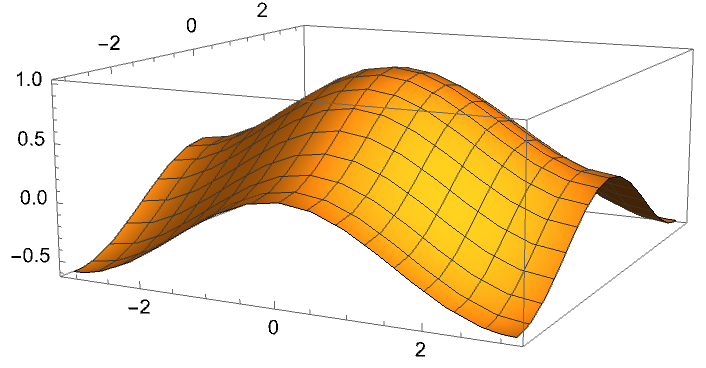
\includegraphics[scale=0.8]{q1b.png}
				\end{center}
			\end{solution}
	\end{enumerate}
	\pagebreak
	\section*{Problem 2}
	In general, computers store images as a 2-dimensional array of pixels, which we will represent as a 2-dimensional
	signal \( z[n_1, n_2 ] \). Given an image, we can apply filters to change its appearance (for instance, blurring 
	or sharpening an image). In this problem, we will examine one of these filters in the frequency domain. 

	Let's consider the following 4-point moving average filter. 
	\[
		h_1[n_x, n_y] = \frac{1}{4}(\delta[x,y] + \delta[x, y-1] + \delta[x - 1, y] + \delta[x-1, y-1])
	\] 
	\begin{enumerate}[label=\alph*)]
		\item Is the function \( h_1[n_x, n_y] \) separable?

			\begin{solution}
				This is indeed separable:
				\[
					h_1[n_x, n_y] = \frac{1}{4}(\delta_x[x] + \delta_x[x - 1])(\delta_y[y] + \delta_y[y-1])
				\] 
			\end{solution}
		\item Find the frequency response \( H(e^{j \omega_x}, e^{j \omega_y}) \) of the filter. 

			\begin{solution}
				The frequency response is given by the Fourier transform of \( h_1[n_x, n_y] \). Because the 
				Fourier transform of delta functions is just an exponential, the algebra is quite easy:
				\[
				H(e^{j \omega_x}, e^{j \omega_y}) = \frac{1}{4}(1 + e^{-j \omega_x x})(1 + e^{-j \omega_y y})
				= e^{-j \omega_x / 2} e^{-j \omega_y / 2} \cos(\omega_x / 2)\cos(\omega_y / 2)
				\] 
			\end{solution}
		\item What type of filter is this? What frequencies pass through without being 
			attenuated?

			\begin{solution}
				Because this is a discrete-time signal, the frequencies are \( 2\pi \)-periodic, meaning that 
				we only need to consider the region between \( 0 \) and \( 2\pi \) in order to find out what kind of 
				filter this is. Because they're cosines, we can then conclude that 
				this is a low-pass filter. 
			\end{solution}
		\item Find the magnitude and phase of \( H_1(e^{j \omega_x}, e^{j0}) \). 

			\begin{solution}
				Here we plug in \( y = 0 \), so the function looks like:
				\[
				H_1(e^{j \omega_x}, e^{j 0}) = e^{-j \omega_x / 2}\cos(\omega_x / 2)
				\] 
				Here, the cosine is real-valued so:
				\[
				|H_1| = \cos(\omega_x / 2) \quad \angle H_1 = \omega_x / 2
				\] 
			\end{solution}
		\item Let's say you have an image represented by the signal
			\[
				z[n_x, n_y] = \frac{1}{2}\cos\left[ \frac{\pi}{2}n_x \right] \sin\left[ \frac{\pi}{3}n_y \right] 
				+ \frac{1}{2}
			\] 
			If you apply the filter \( h_1[n_x, n_y] \) to \( z \), what is the resulting image 
			\( z_1[n_x, n_y] = (z * h_1)[n_x, n_y] \)?

			\begin{solution}
				The 2D convolution in question is:
				\[
					\sum_{m_1, m_2} \frac{1}{2}\left( \cos \left[ \frac{\pi}{2}m_1 \right] \sin\left[ \frac{\pi}{3}m_2 \right] + 1 \right) \cdot \frac{1}{4}(\delta_x [x - m_1] + \delta_x[x - 1 - m_1])(\delta_y[y - m_2] + \delta_y[y - 1 - m_2])
				\] 
				We can expand everything out, and notice that we will get 4 terms, one for every combination of 
				delta functions. 
				\begin{dmath*}
					z_1[n_x, n_y] = \frac{1}{8}\left[
						 \left(\cos\left[ \frac{\pi}{2}n_x \right] \sin\left[ \frac{\pi}{3}n_y \right] + 1\right) 
						+ \left( \cos\left[ \frac{\pi}{2}(n_x -1) \right] \sin\left[ \frac{\pi}{3}n_y \right] + 1 \right) \\
						+ \left( \cos\left[ \frac{\pi}{2}n_x \right] \sin\left[ \frac{\pi}{3}(n_y - 1) \right] + 1 \right) 
						+ \left( \cos\left[ \frac{\pi}{2}(n_x - 1) \right] \sin\left[ \frac{\pi}{3}(n_y - 1) \right] + 1 \right) \right]
				\end{dmath*}
				This simplifies a little if we combine some terms:
				\begin{dmath*}
					z_1[n_x, n_y] = \frac{1}{8}\left[ \cos \left[ \frac{\pi}{2}n_x \right] 
					\sin\left[ \frac{\pi}{3}n_y \right] + \cos\left[ \frac{\pi}{2}(n_x - 1) \right] 
				\sin \left[ \frac{\pi}{3}n_y \right] + \\ \cos\left[ \frac{\pi}{2}n_x \right] 
			\sin\left[ \frac{\pi}{3}(n_y - 1) \right] + 
		\cos\left[ \frac{\pi}{2}(n_x - 1) \right] \sin\left[ \frac{\pi}{3}(n_y - 1) \right] + 4\right] 
			\end{dmath*}
			\end{solution}
		\item Describe qualitatively what a moving average filter does to an image. 

			\begin{solution}
				As far as I can tell based on the equations, a moving average filter basically just smoothens 
				out the image, and (as its name suggests), every pixel's intensity now reflects the average 
				intensity of the pixels around it. 

				As a total effect, this basically corresponds to the image ``smoothening out'' and looking overall 
				more uniform.
			\end{solution}
	\end{enumerate}
	\pagebreak
	\section*{Problem 3}
	The theorem of computed tomography is based on ``Projection-slice Theorem" (a.k.a. ``Central-slide Theorem'', 
	a.k.a. ``Fourier-slice Theorem''). It is a widely used application of 2d FT. In the 2D case, Projection-slice 
	Theorem states: The 1D Fourier transform of a projection at angle \( \theta \) is the 2D Fourier transform 
	of the object evaluated at angle \( \theta \).
	\[
	\mathcal F_{1D}\{p(l; \theta)\}  = \mathcal F_{2D}\{f(x, y)\} (\rho, \theta)
	\] 
	Prove this theorem. 

	\begin{solution}
		I will provide the solution I private-posted on EdStem, not sure if it's correct but it's been 3 days 
		since the post without reply (I'm also inclined to give myself full points for this solution until I'm 
		told otherwise that the proof is wrong). 

		In essence, instead of performing the computations in the \( (x, y) \) plane, we will instead consider 
		the Fourier transform and computations in a rotated \( (x', y') \) frame, tilted at the angle 
		\( \theta \). In this frame, the projection is computed as:
		\[
		\rho = \int_{-\infty}^{\infty} f(x', y') dy' 
		\] 
		then the Fourier transform of this is computed as:
		\[
		\mathcal F_{\text{1D}}\{\rho\}  = \int_{-\infty}^{\infty} \int_{-\infty}^{\infty} 
		f(x', y') \diff y' e^{-j \omega_x x'} \diff x' = \int_{-\infty}^{\infty} 
		\int_{-\infty}^{\infty} f(x', y') e^{-j \omega_x x'} \diff x' \diff y'
		\] 
		As for the 2DFT, because this basis is also orthogonal, the form of the Fourier transform doesn't 
		change:
		\[
		\mathcal F_{\text{2D}}\{f(x', y')\} = \int_{-\infty}^{\infty} \int_{-\infty}^{\infty} 
		f(x', y') e^{-j \omega_x x'} e^{-j \omega_y y'} \diff x' \diff y'
		\] 
		Now, evaluation at an angle \( \theta \) now means evaluating about the line \( \omega_y = 0 \), so therefore 
		we have:
		\[
		\mathcal F_{\text{2D}}\{f(x', y')\}(\rho, \theta) = \int_{-\infty}^{\infty} \int_{-\infty}^{\infty} 
		f(x', y') e^{-j \omega_x x'} \diff x' \diff y'
		\] 
		which matches the equation for \( \mathcal F_{\text{1D}}\{\rho\}  \), and completes the proof. 
	\end{solution}
	\pagebreak
	\section*{Problem 4}
	In the olden days of Spring 2021, the professor asked what te Fourier transform of the curtain behind DiCaprio 
	would look like. We will address this now. 

	It is a 2 dimensional (2D) image, so we need to use the 2DFT. In this question, we use linear frequency without 
	loss of generality. Recall the 2DFT of a 2D function \( f(x, y) \) is:
	\begin{align*}
		F(f_x, f_y) &= \int_{-\infty}^{\infty} \int_{-\infty}^{\infty} f(x, y) e^{-j 2\pi(f_x x + f_yy)}
		\diff x \diff y & \text{(2DFT)}\\
		f(x, y) &= \int_{-\infty}^{\infty} \int_{-\infty}^{\infty} F(f_x, f_y) e^{j 2\pi (f_x x + f_y y)}
		\diff f_x \diff f_y & \text{(inverse 2DFT)}
	\end{align*}
	In this problem, we consider real-valued \( f(x, y) \). 
	\begin{enumerate}[label=\alph*)]
		\item Compute and sketch the magnitude of 2D FT of the following patterns:
			\begin{itemize}
				\item \( f(x, y) = 1 \) 

					\begin{solution}
						\begin{center}
							\begin{tikzpicture}[scale=2]
								\draw (-1, 0) -- (1, 0) node[right] {\( f_x \) };
								\draw (0, -1) -- (0, 1) node[right] {\( f_y \) };
								\filldraw[red] (0,0) circle (.3mm);
							\end{tikzpicture}
						\end{center}
					\end{solution}
				\item \( f(x, y) = \sin \frac{2\pi}{100} x \) 

					\begin{solution}
						This is a sinusoid, so we just have two delta functions along \( x \) at the 
						appropriate frequencies:
						\begin{center}
							\begin{tikzpicture}[scale=2]
								\draw (-1, 0) -- (1, 0) node[right] {\( f_x \) };
								\draw (0, -1) -- (0, 1) node[right] {\( f_y \) };
								\filldraw[red] (-0.2,0) circle (.3mm) node[above left] {\small{\( (-0.01, 0) \) }};
								\filldraw[red] (0.2, 0) circle (.3mm) node[above right] {\small{\( (0.01, 0) \) }};
							\end{tikzpicture}
						\end{center}
						Note that we have \( 0.01 \) here because the frequency is \( \frac{1}{100} \). 
					\end{solution}
				\item \( f(x, y) = \sin(\frac{2\pi}{100} x + \frac{2\pi}{100} y) \) 

					\begin{solution}
						Here, we will have two delta functions shifted by the combination 
						\( \frac{2\pi}{100}x + \frac{2\pi}{100y} \) and \( -\frac{2\pi}{100}x - \frac{2\pi}{100}y \), 
						so this will give us:
						\begin{center}
							\begin{tikzpicture}[scale=2]
								\draw (-1, 0) -- (1, 0) node[right] {\( f_x \) };
								\draw (0, -1) -- (0, 1) node[right] {\( f_y \) };
								\filldraw[red] (0.1,0.1) circle (.3mm) node[above right] {\small{\((0.01, 0.01) \) }};
								\filldraw[red] (-0.1, -0.1) circle (.3mm) node[below left] {\small{\( (-0.01, -0.01) \) }};
							\end{tikzpicture}
						\end{center}
						I included the coordinates in decimals just becuase it was easier for me, and that remains 
						true for the preceding subparts.  
					\end{solution}
				\item \( f(x, y) = \sin(\frac{2\pi}{50} x + \frac{2\pi}{100} y) \) 

					\begin{solution}
						\begin{center}
							\begin{tikzpicture}[scale=2]
								\draw (-1, 0) -- (1, 0) node[right] {\( f_x \) };
								\draw (0, -1) -- (0, 1) node[right] {\( f_y \) };
								\filldraw[red] (0.2,0.1) circle (.3mm) node[above right] {\small{\((0.02, 0.01) \) }};
								\filldraw[red] (-0.2, -0.1) circle (.3mm) node[below left] {\small{\( (-0.02, -0.01) \) }};
							\end{tikzpicture}
						\end{center}
					\end{solution}
				\item \( f(x, y) = \sin(\frac{2\pi}{20} x + \frac{2\pi}{40} y) \)

					\begin{solution}
						\begin{center}
							\begin{tikzpicture}[scale=2]
								\draw (-1, 0) -- (1, 0) node[right] {\( f_x \) };
								\draw (0, -1) -- (0, 1) node[right] {\( f_y \) };
								\filldraw[red] (0.5,0.25) circle (.3mm) node[above right] {\small{\((0.05, 0.025) \) }};
								\filldraw[red] (-0.5, -0.25) circle (.3mm) node[below left] 
									{\small{\( (-0.05, -0.025) \) }};
							\end{tikzpicture}
						\end{center}
					\end{solution}
			\end{itemize}
		\item Now we consider the illumination situation in the picture. We then model the luminosity of one light 
			source follows:
			\[
				I(r) = I_0e^{-ar^2}
			\] 
			where \( I_0 \) is the intensity of light at the source, \( r \) is the distance from 
			the light source, \( r^2 = x^2 + y^2 \). 
			
			Find the 2D FT of Gaussian \( h(x, y) = e^{-a(x^2 + y^2)} \) where \( a > 0 \). What 
			shape is this? 

			\begin{solution}
				This is a separable equation:
				\[
				e^{-a(x^2 + y^2)} = e^{-ax^2} e^{-ay^2}
				\] 
				meaning that the 2D Fourier transform will also be a product. Also, because they're the same form, 
				we'll just get two copies of the same function. Calculating one of them:
				\[
				\mathcal F \{e^{-ax^2}\}  = \int_{-\infty}^{\infty} e^{-ax^2}e^{-2 \pi j f_x x} \diff x 
				\] 
				This is a well known integral, I proved in homework 6 that:
				\[
				\int_{-\infty}^{\infty} e^{-\frac{a}{2}x^2 + bx} = e^{\frac{b^2}{2a}}\sqrt{\frac{2\pi}{a}}  
				\] 
				(the proof just involves change of variables) so applying it to this equation, we have:
				\[
				\mathcal F \{e^{-ax^2}\} = e^{-\pi^2 f_x^2 / a}\sqrt{\frac{\pi}{a}} 
				\] 
				Thus, the full Fourier transform is:
				\[
				H(\omega_x, \omega_y) =\frac{\pi}{a} e^{-\pi^2 f_x^2 / a}e^{-\pi^2 f_y^2 / a}
				\] 
				This is a 2-dimensional Gaussian. 
			\end{solution}
		\item We model the curtain behind him to be \( f(x,y) = \sin(\frac{2\pi}{10} x) \cos(\frac{2\pi}{50} y) \).
			What's the 2D FT of this curtain pattern?

			\begin{solution}
				Again, this is separable, so we just have a product over \( x \) and \( y \). The Fourier 
				transform of sines and cosines are just linear combinations of plane 
				waves with the positive and negative 
				frequency (with appropriate prefactors), so we have:
				\[
					F(f_x, f_y) = \frac{1}{4i}\left( \delta\left(f_x - \frac{2\pi}{10}\right) - 
				\delta\left( f_x + \frac{2\pi}{10} \right) \right) 
				\left( \delta\left( f_y- \frac{2\pi}{50} \right) + 
				\delta\left( f_y + \frac{2\pi}{50} \right)  \right) 
				\] 
			\end{solution}
		\item Suppose the light source is at the center of the frame. What is the 2D FT of the pattern from 
			part 3. with centered light source with \( a = 1 \) from part (b)?
			\begin{enumerate}[label=\roman*)]
				\item Show that 
					\[
					\mathcal F \{f(x, y) \cdot g(x, y) \}  = F(f_x, f_y) * G(f_x, f_y)
					\] 
					for any aribtrary \( f(x, y) \) and \( g(x, y) \) with corresponding Fourier 
					transform \( F(f_x, f_y) \) and \( G(f_x, f_y) \). 

					\begin{solution}
						I will instead prove the inverse relation:
						\[
						f(x, y) \cdot g(x, y) = \mathcal F^{-1}\{F(f_x, f_y) * G(f_x, f_y)\} 
						\] 
						The inverse Fourier transform of the convolution is written as:
						\[
						\int_{-\infty}^{\infty} \int_{-\infty}^{\infty} \int_{-\infty}^{\infty} \int_{-\infty}^{\infty} 
						F(f_x', f_y') G(f_x - f_x', f_y - f_y') e^{2 \pi j f_x}e^{2\pi j f_y}\diff f_x
						\diff f_y \diff f_x' \diff f_y'
						\] 
						We can then rearrange it as follows:
						\[
						\int_{-\infty}^{\infty} \int_{-\infty}^{\infty} F(f_x', f_y') 
						\left( \int_{-\infty}^{\infty} \int_{-\infty}^{\infty} G(f_x- f_x', f_y - f_y')
						e^{j 2 \pi f_x}e^{2 \pi j f_y} \diff f_x \diff f_y \right) 
						\diff f_x' \diff f_y'
						\] 
						We can then use the property that: \( X(f - f_0) \leftrightarrow e^{2 \pi j f_0t}x(t) \)
						to simplify the expression in parentheses:
						\[
						\int_{-\infty}^{\infty} \int_{-\infty}^{\infty} G(f_x - f_x', f_y - f_y') 
						e^{2 \pi j f_x}e^{2 \pi j f_y} \diff f_x \diff f_y = g(x, y) e^{2 \pi j f_x'}e^{2 \pi j f_y'}
						\] 
						Therefore, the equation now becomes:
						\[
						g(x, y)\underbrace{ \int_{-\infty}^{\infty} \int_{-\infty}^{\infty} 
						F(f_x', f_y') e^{2 \pi j f_x'}e^{2 \pi j f_y'} \diff  x' \diff y'}_
						{f(x, y)}= f(x, y) \cdot g(x, y)
						\] 
						where the \( \cdot \) denotes pointwise multiplication.
					\end{solution}
				\item Find the 2D FT of \( f(x, y) \cdot h(x, y) \)

					\begin{solution}
						Here, we will use the 2D convolution theorem to help us, since the Fourier transform is 
						just a convolution in frequency space.   

						Because \( F(f_x, f_y) \) is a series of delta functions, this is relatively easy. 
						We know that the convolution has the property that \( x(t) * \delta( t - T) = 
						x(t - T)\), so this means that we will basically have four terms that are just a 
						combination of the shifts:
						\begin{dmath*}
							Y(f_x, f_y) = \frac{\pi}{4ai}
							\left[ e^{-\pi^2 \left( f_x - \frac{2\pi}{10} \right)^2 / a} 
							e^{-\pi^2 \left( f_y - \frac{2\pi}{50} \right)^2} 
							+ e^{-\pi^2 \left( f_x - \frac{2\pi}{10} \right)^2}
							e^{-\pi^2\left( f_y + \frac{2\pi}{50} \right)^2}\\
							- e^{-\pi^2\left( f_x + \frac{2\pi}{10} \right)^2} 
							e^{-\pi^2\left( f_y - \frac{2\pi}{50} \right)^2}
							- e^{-\pi^2\left( f_x + \frac{2\pi}{10} \right)^2}
							e^{-\pi^2 \left( f_y + \frac{2\pi}{50} \right)^2}
						\right] 
						\end{dmath*}
					\end{solution}
			\end{enumerate}
		\item Finally, we can answer the question: ``What would the Fourier transform of the curtain 
			behind DiCaprio look like'' Hint: The light source seems to be on the right hand side of the image.  

			\begin{solution}
				If the light source is not centered, then this is the same as basically shifting 
				\( h(x, y) \), so that we have \( h(x - x_0, y - y_0) \). In terms of a Fourier transform, we can use 
				the relation that:
				\[
				\mathcal F \{h(x - x_0, y - y_0)\}  = e^{-j \omega x_0}e^{-j \omega y_0} \mathcal F \{h(x, y)\} 
				\] 
				this is the two-dimensional version of the time-shift property. So depending on the location (say, 
				the source was located at \( (x_0, y_0) \)), we 
				basically have:
				\begin{dmath*}
					Y(f_x, f_y) = e^{-2 \pi j (f_x x_0 + f_y y_0)}\frac{\pi}{4ai}
					\left[ e^{-\pi^2 \left( f_x - \frac{2\pi}{10} \right)^2 / a} 
					e^{-\pi^2 \left( f_y - \frac{2\pi}{50} \right)^2} 
					+ e^{-\pi^2 \left( f_x - \frac{2\pi}{10} \right)^2}
					e^{-\pi^2\left( f_y + \frac{2\pi}{50} \right)^2}\\
					- e^{-\pi^2\left( f_x + \frac{2\pi}{10} \right)^2} 
					e^{-\pi^2\left( f_y - \frac{2\pi}{50} \right)^2}
					- e^{-\pi^2\left( f_x + \frac{2\pi}{10} \right)^2}
					e^{-\pi^2 \left( f_y + \frac{2\pi}{50} \right)^2}
				\right] 
				\end{dmath*}

			\end{solution}
	\end{enumerate}
\end{document}
